\section{文档}

\subsection{框架}

    \begin{frame}[fragile]
        \begin{itemize}
            \item 你书写的是包含LaTeX代码和实际内容的纯文本文件(.tex文件)。
            \item LaTeX代码控制实际内容的格式和样式。
        \end{itemize}
    \end{frame}

	\begin{frame}[fragile]
\begin{lstlisting}
% xiaoming.tex
% 注释说明
\documentclass[UTF8]{ctexart} % 文档类型
\title{食谱}
\author{小明}
\date{\today}                 % 以上为“导言区”
\begin{document}              % 文档开始
% document内的内容可与pdf文件一一对应!
\maketitle
现作出如下声明
\begin{itemize}
    \item 不吃胡萝卜
    \item 豆花只吃甜的
\end{itemize}
\end{document}                % 以上为“正文区”
\end{lstlisting}
	\end{frame}


\subsection{两个必要元素}%hbk
	\begin{frame}[fragile]
	    \frametitle{documentclass}
		\begin{itemize}
			\item documenclass,文档类,是第一个必要元素:\\
			写的是什么,怎样排版
\begin{lstlisting}
\doucumentclass[·]{·}
% 方括号内为可选项,可设置纸张大小,字体大小,纸张方向,编码方式,草稿定稿,单双面等属性
\end{lstlisting}\pause
			\item 常用标准文档:\\
			article, book, report, letter, beamer (前三者为基本文档类;ctex宏集了解一下)
			\item cls文件:\\
			自定义的文档类型(CUMCMThesis-master)
		\end{itemize}
	\end{frame}
	
    \begin{frame}
        \frametitle{document}
        document环境是一份tex文档的第二个必要元素,其内为pdf文件的具体内容\pause
\begin{figure}
\centering
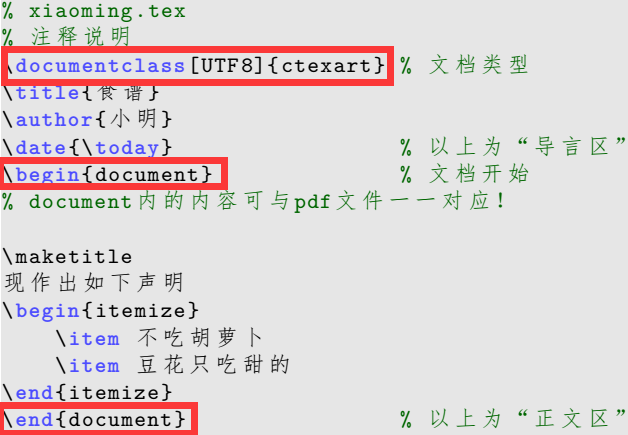
\includegraphics[width = 0.7\textwidth]{img//nece.png}
\end{figure}
    \end{frame}


\subsection{环境}
    \begin{frame}[fragile]
        \frametitle{什么是环境}
        \begin{itemize}
            \item 你也许注意到了\verb|\begin|和\verb|\end| \pause
            \item \verb|\begin|和\verb|\end|语句不是命令,而是对环境进行了定义。
            \item begin和end间的环境,代表这块区间应用的\textbf{排版}规则
            \item 可以多个环境层层嵌套(不可交叉!)
        \end{itemize}
    \end{frame}
    
    \begin{frame}[fragile]
\begin{lstlisting}
% 正确用法:

\begin{document}
  \begin{environment1}
    \begin{environment2}
    \end{environment2}
  \end{environment1}
\end{document}

% 错误用法:

\begin{document}
  \begin{environment1}
    \begin{environment2}
  \end{environment1}
    \end{environment2}
\end{document}
\end{lstlisting}
    \end{frame}
    
    
	\begin{frame}[fragile]
		\begin{itemize}
			\item 模块化与环境的思想\\
			打开 "environment\_cmp.tex"
			\item 为什么section2每一行都居中了?
			\item 你能不能通过添加环境的方式,让section2第一行靠左?(提示:flushleft)
			\item 这是否引发了你对优先级的思考?
		\end{itemize}
	\end{frame}
	
	
\subsection{字体}
    \begin{frame}
        \frametitle{问题}
        \begin{itemize}
            \item 字体太丑,或者有字体要求(如Times New Roman,俄语,德语)
            \item 字体颜色
            \item 键盘无法输入的符号(如$\pi$, \AA, $^{\circ}$C)
            \item 貌似可以用键盘输入的符号(如\%, \{, $\sim$)
            \item 其他(空格:\fbox{\$\qquad\$}, \fbox{\$\quad\$}, \fbox{\$\ \$}, \fbox{\$\;\$}, \fbox{\$~\$} \fbox{\$\,\$}, \fbox{\$\!\$})
        \end{itemize}
    \end{frame}

    \begin{frame}
        \frametitle{解决方法}
        \begin{itemize}
            \item 了解相关的宏包,以及相关命令设置,如fontspec,babel等等
            \item 要用去网上查
            \item 看手册(已准备好,在LM文件夹里)
            \item 以上两条也针对其他琐碎的细节,如字号、行距、盒子等等
        \end{itemize}
    \end{frame}